\section{Introduction to Trees}\label{sec:introduction_to_trees}

Sometimes trees appear in the natural world like in a family tree for example, but this dynamic data structure can also create a \emph{binary search tree} instead of a linear array to search for a particular element in a collection.

\subsection{Binary Search Tree}\label{sub:binary_search_tree}

To search through an array of \(n\) elements to find a particular element, the time complexity is \(O(n)\), but using a binary search tree we can reduce this to \(O(\log_2 n)\) because at each size we can cut down the size of the problem by half.

\begin{highlight}{A binary search tree}
    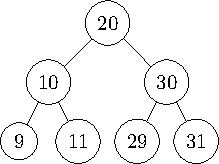
\includegraphics{lualatex/pa/8/binarysearchtree.pdf}
\end{highlight}

\paragraph{Linear}\label{par:linearbst}

For the linear search, we are counting how many steps it takes to reduce \(n\) to \(1\) by decrementing by \(1\).

\paragraph{Logarithmic}\label{par:logarithmicbst}

For the binary search tree, we are counting how many steps it take to reduce \(n\) to \(1\) by halving each time.

\subsubsection{Uses}\label{ssub:usesbst}

Often information lends itself to the tree structure automatically, some examples are:
\begin{itemize}
    \item Family trees
    \item Biology classification trees
    \item File systems
    \item Web addresses
\end{itemize}
However, data doesn't always fall into that structure, but we can force the data into that structure because of the algorithmic complexity gains.

\subsection{Basic Definitions}\label{sub:basic_definitions}

\begin{description}
    \item[Node] Each value on a tree
    \item[Edge] Edges connect two nodes together in one direction
    \item[Root] The very top node without any other nodes pointing to it
    \item[Path] The edges and nodes that you have to take to go from one node to another node
    \item[Children] All direct descendants of another node
    \item[Parent] The node that another node is connected to
    \item[Sibling] All nodes that are children of the same parent
    \item[Subtree] Any node and all of its descendants can form a subtree inside a larger tree
    \item[Leaf node] Nodes that have no descendants
    \item[Level] How many steps it is from the root
    \item[Height] The total number of levels on a tree
\end{description}

\subsection{Definition}\label{sub:definitiontree}

A tree is:
\begin{itemize}
    \item A \emph{set} of nodes
    \item A \emph{set} of edges that connect pairs of nodes
\end{itemize}
such that:
\begin{itemize}
    \item One node is the root node
    \item Every node (except root) is connected by an edge from only one other node (eg. Every node has one parent)
    \item There is a unique path from root to every node (comes from every node having one parent)
    \item A node can have any number of children, but a tree can only be called a \emph{binary tree} if each node has a maximum of two children.
\end{itemize}

\begin{note}
    A tree is a recursive data structure since every node of a tree can be considered the root of another sub tree.
    This recursive nature lends itself to recursive operations very well.
\end{note}

\section{Binary Trees and Balanced Binary Trees}\label{sec:binary_trees_and_balanced_binary_trees}

A binary tree is a linked data structure where each node has a \mintinline{text}{key} attribute, and three pointer attributes:
\begin{itemize}
    \item \mintinline{text}{node.p} points to the parent
    \item \mintinline{text}{node.left} points to the left child
    \item \mintinline{text}{node.right} points to the right child
\end{itemize}
Where the child or parent is missing (we are at the root, or there is only one child), we set the value to \mintinline{text}{NILL}.

\subsection{Balanced Binary Trees}\label{sub:balanced_binary_trees}

\begin{highlight}{A balanced binary search tree compared with an unbalanced binary tree}
    \begin{minipage}{0.45\linewidth}
        \centering
        A balanced binary tree

        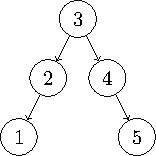
\includegraphics{lualatex/pa/8/balancedbst.pdf}
    \end{minipage}
    \hfill
    \begin{minipage}{0.45\linewidth}
        \centering
        An unbalanced binary tree

        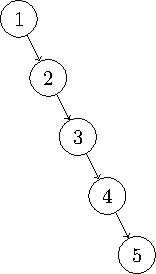
\includegraphics{lualatex/pa/8/unbalancedbst.pdf}
    \end{minipage}
\end{highlight}

A balanced tree is where the left and right subtrees of very node differ in height by no more than \(1\), making the total time complexity to traverse the tree \(O(\log n)\).

Where we have an extremely unbalanced tree, it is pretty much a linked list, so the time complexity is \(O(n)\)
\begin{note}
    Generally graph algorithms work better on a balanced tree.
\end{note}

\section{Traversing a Tree}\label{sec:traversing_a_tree}

When you traverse (or walk) a tree, you visit each node exactly one.
Where is no single obvious way to go through a tree like there was with a linked list.
There are two types of traversal:
\begin{description}
    \item[Breadth-first] We are most occasionally interested in going through each level at a time. Sometimes called \emph{level-order traversal}.
    \item[Depth-first] Most often we are interested in going down each branch before going down the next.
\end{description}

\subsection{Breadth First}\label{sub:breadth_first}

\begin{highlight}{The order of nodes visited in the breadth first traversal of a binary tree}
    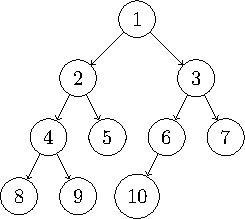
\includegraphics{lualatex/pa/8/breadthfirst.pdf}
\end{highlight}

Level traversal isn't always enough because it loses all of the ordering of the branches.

\subsubsection{Inorder Traversal}\label{ssub:inorder_traversal}

For an \emph{inorder traversal}, you first go to the leftmost leaf node, then you work your way back up to the top again recording the value of the parent (which wasn't technically visited on the way down), the left node, and then the right, so the order for any subtree is:
\begin{enumerate}
    \item Parent
    \item Left child
    \item Right child
\end{enumerate}
\begin{code}{text}
    INORDER(node)
        if node != NILL
            INORDER(node.left)
            print node.key
            INORDER(node.right)
\end{code}

\begin{highlight}{The order of nodes visited in the inorder traversal of a binary tree}
    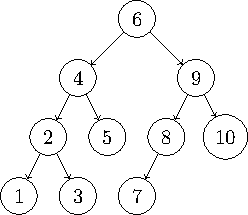
\includegraphics{lualatex/pa/8/inordertraversal.pdf}
\end{highlight}

\subsubsection{Preorder Traversal}\label{ssub:preorder_traversal}

For a \emph{preorder traversal}, you travel down through each left node recording the value each time, continuing until you reach then leaf node, then continue back up again visiting the right hand nodes, so the final order is:
\begin{enumerate}
    \item Parent
    \item Left child and all left hand descendants
    \item Right child and all right hand descendants
\end{enumerate}
\begin{code}{text}
    PREORDER(node)
        if node != NILL
            print node.key
            PREORDER(node.left)
            PREORDER(node.right)
\end{code}

\begin{highlight}{The order of nodes visited in the preorder traversal of a binary tree}
    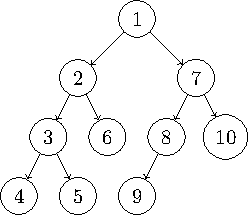
\includegraphics{lualatex/pa/8/preordertraversal.pdf}
\end{highlight}

\subsubsection{Postorder Traversal}\label{ssub:postorder_traversal}

For a \emph{postorder traversal}, you first go to the leftmost leaf node, then you work your way back up to the top again recording the value of the left node, then the parent node (which wasn't technically visited on the way down), and then the right, so the order for any subtree is:
\begin{enumerate}
    \item Left child
    \item Parent
    \item Right child
\end{enumerate}
\begin{code}{text}
    INORDER(node)
        if node != NILL
            INORDER(node.left)
            INORDER(node.right)
            print node.key
\end{code}

\begin{highlight}{The order of nodes visited in the postorder traversal of a binary tree}
    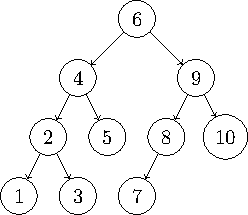
\includegraphics{lualatex/pa/8/postordertraversal.pdf}
\end{highlight}

\subsubsection{Recursive}\label{ssub:recursivetreetraversal}

Recursive algorithms are a very well known pattern that works by making a function call itself until some \emph{terminating condition} is met.
All of these depth first traversals are defined recursively because a tree is a recursive data structure.

\section{Binary Search Tree}\label{sec:binary_search_tree_operations}

A binary search tree is simply a binary tree where:
\begin{itemize}
    \item All nodes on the left subtree have keys smaller than \mintinline{text}{node.key}
    \item All nodes on the right subtree have keys larger than \mintinline{text}{node.key}
\end{itemize}
We can use an inorder traversal to get an ordered sequence.

Searching through a regular tree is time complexity \(O(n)\), but using a binary search tree means the time complexity is \(O(\text{height})\) which is roughly equal to \(O(\log n\) if the tree is perfectly balanced.
\begin{note}
    Remember: each step we eliminate half of the tree.
\end{note}

\section{Operations on Binary Search Trees}\label{sec:operations_on_binary_search_trees}

A binary search tree stored data in a specific structure, but to make the structure work for us, we need to define algorithms to perform operations on it (like we did for linked lists earlier).
The time complexity of all of the operations will be \(O(\text{height})\) where the height of a balanced tree is \(\log n\).

\subsection{Search}\label{sub:searchbst}

If the value we are looking for exists, we want to return a pointer to the while node, and return \mintinline{text}{NILL} otherwise.
\begin{code}{text}
    SEARCH(node, key)
        if node.key == key OR node == NILL
            return node
        if node.key > key
            return SEARCH(node.left)
        else
            return SEARCH(node.right)
\end{code}
Although this is a recursive function, we can also implement it recursively, which is usually more efficient.
\begin{code}{text}
    SEARCH-ITER(node, key)
        while node != NILL AND node.key != key
            if key < node.key
                node = node.left
            else
                node = node.right
\end{code}

\subsection{Insert}\label{sub:insertbst}

When we insert to a binary search tree, there are two steps:
\begin{enumerate}
    \item Create node
    \item Find an appropriate empty slot (remember it must still be a binary search tree).
    \item Insert the node to the position (remember to keep track of the \mintinline{text}{pnode} so that you can set \mintinline{text}{inode.parent} properly).
\end{enumerate}

\begin{code}{text}
    cnode = tree.root # current node
    pnode = NILL # parent node

    while cnode != NILL # leaf node has been found
        pnode = cnode
        if inode.key < cnode.key
            cnode = cnode.left
        else
            cnode = cnode.right

    inode.parent = pnode

    if pnode == NILL # We are at the root
        tree.root = inode
    elif inode.key < pnode.key
        pnode.left = inode
    else
        pnode.right = inode
\end{code}

\subsection{Minimum and Maximum}\label{sub:minimum_and_maximumbst}

Finding the minimum and maximums is very easy since we know that every node on the left of the parent is less than the parent, and that every node on the right is greater than the parent meaning that we can find the leftmost node for the minimum and rightmost node for the maximum.

\subsection{Linked List Implementation}\label{sub:linked_list_implementation}

A linked list is already a stack really, where the end pointer is points to the top pointer, since there is no traversal, we can say that the time complexity is \(O(1)\).
\begin{description}
    \item[PUSH] Insert to head
    \item[POP] Delete head, return value
\end{description}
\begin{note}
    Remember, we still need to prevent underflows
\end{note}

\section{Limitations of Binary Search Trees}\label{sec:limitations_of_binary_search_trees}

Each basic operation on a binary tree runs on \(O(h)\), but height varies as nodes are added or removed which can be problematic if the tree is not kept balanced (it could end up basically a linked list).
We should use \emph{self-balancing trees} where some extensions have been added to the basic binary search tree definition:
\begin{itemize}
    \item Red-black trees
    \item AVL trees
    \item B-trees
\end{itemize}
A common method to keep the tree balanced is to perform a rotation (basically tidying up / house keeping) after each deletion or insertion.
When we rotate, we find a pivot, then we swap to parent to the child so that the pivot is now the parent.

\section{Queue}\label{sec:paeightqueue}

For a queue, you enqueue and dequeue from the queue, where enqueuing adds nodes to the tail (the end), and dequeuing removes from the head (the front) of the list.

As with a stack, we have a ``peek'' called \mintinline{text}{FRONT-OF-QUEUE} that returns the front value, but doesn't remove it.
\mintinline{text}{SIZE-OF} returns the size, and \mintinline{text}{EMPTY} also returns whether the queue is empty or not.
\begin{note}
    Dequeuing an empty queue will still underflow.
\end{note}

If we were to implement a queue using an array, we have the head pointing to the start of the array, so when we dequeue from the queue, we have to move the head pointer forwards by one place, which unfortunately means we lose one place worth of space (we might even run out of space if the queue is empty).

We must use circular arrays to solve this problem, where we set our array indexes to \mintinline{text}{i=(i+1)%n} to loop back around to the start again.

\subsection{Conditions}\label{sub:queueconditions}

\begin{description}
    \item[Empty] The queue is empty is the head index equals the tail index.
    \item[Full] The queue is full if the head is one less than the tail (does equal pointers mean full or empty?). There is a special case for if the head set the start, then the tail will be \mintinline{text}{n-1} if full.
\end{description}
\begin{note}
    The condition we use for empty does mean that we lose a position in the queue.
    You can store \mintinline{text}{n-1} elements in a queue where \mintinline{text}{len(arr)=n}.
\end{note}

\subsection{Enqueue}\label{sub:enqueue}

\begin{code}{python}
    if self.queuefull:
        throw OverflowError
    else:
        self.arr[self.tail] = new
        self.tail = (self.tail + 1) % len(self.arr)
\end{code}

\subsection{Dequeue}\label{sub:dequeue}

\begin{code}{python}
    if self.queueempty:
        throw UnderfullError
    else:
        node = self.arr[self.head]
        self.head = (self.head + 1) % n
        return node
\end{code}

\subsection{Queue Empty}\label{sub:queueempty}

\begin{code}{python}
    return self.head == self.tail
\end{code}

\subsection{Queue Full}\label{sub:queue_full}

\begin{code}{python}
    return (
        (self.head == self.tail + 1) 
        or (self.head == 0 and self.tail == len(self.arr)-1)
    )
\end{code}

\subsection{Performance and Limitations}\label{sub:performance_and_limitations}

\begin{itemize}
    \item Space complexity is always \(O(n)\)
    \item The space must be defined before hand
\end{itemize}
\begin{note}
    For a linked list, we don't need to worry about any circular arrays, since we can just add or remove nodes whenever we want.
\end{note}
